\documentclass[tikz]{standalone}

% \usepackage{newtxtext,newtxmath}

% mytikzset
\usepackage{tikz}
\usetikzlibrary{positioning,arrows,shapes}
\usetikzlibrary{decorations.pathmorphing}
\usetikzlibrary{decorations.markings}
\usetikzlibrary{shapes.arrows, fadings}
\usetikzlibrary{shapes,snakes}
\usetikzlibrary{calc}

\tikzset{
  vector/.style={thick,double,draw=black, postaction={decorate},
    decoration={markings,mark=at position .6 with {\arrow[black,scale=0.4]{triangle 45}}}},
  axial/.style={thick,double,densely dashed,draw=black, postaction={decorate},
    decoration={markings,mark=at position .6 with {\arrow[black,scale=0.4]{triangle 45}}}},
  gluon/.style={decorate, draw=black,
    decoration={coil,aspect=0.3,segment length=5pt,amplitude=3pt}},
  pseudo/.style={thick, dashed, draw=black, postaction={decorate},
    decoration={markings,mark=at position .6 with {\arrow[red,scale=0.5]{triangle 45}}}},
  scalar/.style={thick,draw=black, postaction={decorate},
    decoration={markings,mark=at position .6 with {\arrow[black,scale=0.5]{triangle 45}}}}%,
  % pomeron/.style={thick,draw=black, postaction={decorate},
  % decoration={zigzag,segment length=4,amplitude=.9}}
}


\definecolor{cola}{rgb}{0.9,0.62,0.0}
\definecolor{colb}{rgb}{0.337, 0.706, 0.914 }
\definecolor{colc}{rgb}{0.0, 0.62, 0.451}

\begin{document}
\nopagecolor
  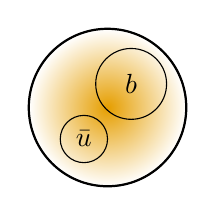
\begin{tikzpicture}[node distance=0.9cm and 1.3cm, baseline=1cm]
    \filldraw[even odd rule,inner color=cola,outer color=white] (0,0) circle (1cm);
    \draw[black,thick] (0,0) circle (1cm);
    \draw[black] (0.3,0.3) circle (4.5mm) node[] {$b$};
    \draw[black] (-0.3,-0.4) circle (3mm) node[] {$\bar{u}$};
    % \fill[black] (c1) circle (1mm);
  \end{tikzpicture}
\end{document}
